\documentclass[Lecture.tex]{subfiles}
\begin{document}
\section{4.1: Local Maxima and Minima}

\begin{frame}
  \begin{defn}
    Let $p$ be a point in the domain of $f$ and let $(a,b)$ be an interval containing $p$.
    \begin{itemize}
    \item<2->
      If $f(p) \leq f(x)$ for every $x$ satisfying $a < x < b$, then $p$ is a {\it local minimum}.
    \item<3->
      If $f(x) \leq f(p)$ for every $x$ satisfying $a < x < b$, then $p$ is a {\it local maximum}.
    \end{itemize}
  \end{defn}
\end{frame}

\begin{frame}{Example}
  \begin{center}
    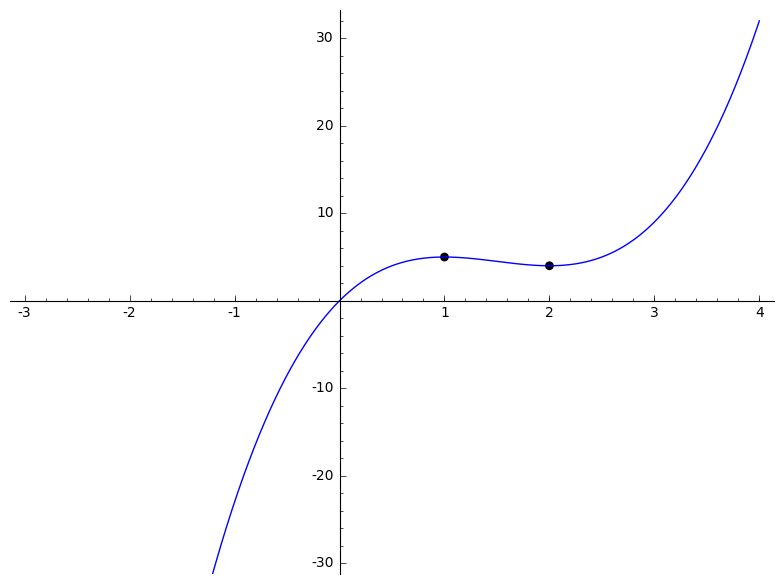
\includegraphics[scale=0.35]{localMinMax}
  \end{center}
  The point on the left is a local minimum, and the point on the right is a local maximum.
\end{frame}

\begin{frame}{Detecting Local Maxima}
  Let $f$ be continuous with continuous derivative, and let $p$ be a local maximum.
  \begin{itemize}
  \item<2->
    To the left of $p$, $f$ is increasing, and to the right of $p$, $f$ is decreasing.
  \item<3->
    Equivalently:
    \begin{center}
      $0 < f^\prime(x)$ for $x < p$
      \quad and \quad 
      $f^\prime(x) < 0$ for $p < x$.
    \end{center}
  \item<4->
    Continuity of $f^\prime$ guarantees that $f^\prime(p) = 0$.
  \end{itemize}
\end{frame}

\begin{frame}{Detecting Local Minima}
  Let $f$ be continuous with continuous derivative, and let $p$ be a local minimum.
  \begin{itemize}
  \item<2->
    To the left of $p$, $f$ is decreasing, and to the right of $p$, $f$ is increasing.
  \item<3->
    Equivalently:
    \begin{center}
      $f^\prime(x) < 0$ for $x < p$ \quad and \quad $0 < f^\prime(x)$ for $p < x$.
    \end{center}
  \item<4->
    Continuity of $f^\prime$ guarantees that $f^\prime(p) = 0$.
  \end{itemize}
\end{frame}

\begin{frame}{Example}
  It's not always true that local extrema occur at zeroes of the first derivative.
  \onslide<2->{
    The absolute value function has a local minimum at $(0,0)$:
  }
  \onslide<3->{
    \begin{center}
      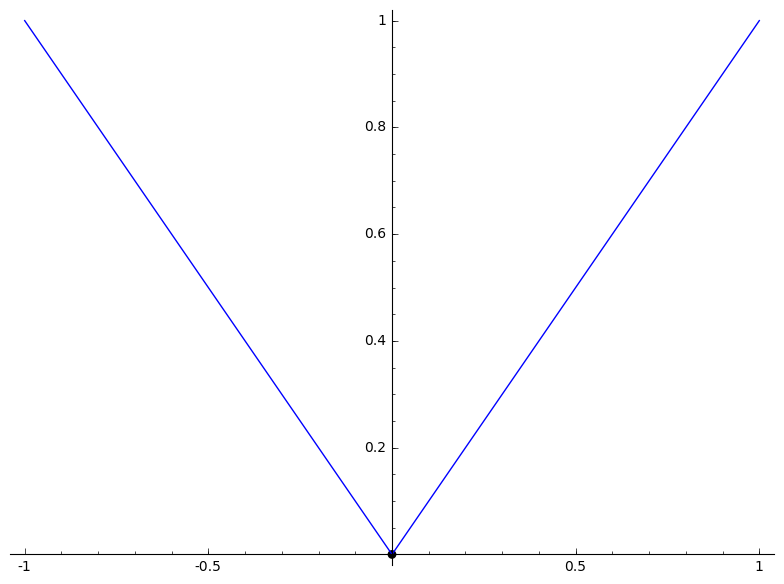
\includegraphics[scale=0.25]{absValMin}
    \end{center}
  }
  \onslide<4->{But the derivative is undefined at 0.}
\end{frame}

\begin{frame}{Critical Points}
  \begin{defn}
    For a function, $f$, a point $p$ in the domain of $f$ is called a {\it critical point} if either
    \begin{itemize}[<+->]
    \item
      $f^\prime(p) = 0$, or
    \item
      $f^\prime(p)$ is undefined.
    \end{itemize}
    \onslide<3->{A critical value of $f$ is the function value, $f(p)$, at a critical point, $p$.}
  \end{defn}
\end{frame}

\begin{frame}{Detecting Local Extrema}
  \begin{thm}
    If a continuous function, $f$, has a local minimum or local maximum at $p$, then $p$ is a critical point of $f$, provided that the domain of $f$ is not a closed interval.
  \end{thm}

\onslide<2->{
  \begin{rmk}
    The converse is {\bf FALSE}.
    The point $x = 0$ is a critical point of $f(x) = x^2$, but neither a local minimum nor a local maximum.
  \end{rmk}
  }
\end{frame}

\begin{frame}{First Derivative Test}
  Let $f$ be a continuous function and let $p$ be a critical point of $f$.
  \begin{itemize}
  \item<2->
    If $f^\prime(x) < 0$ for $x < p$ and $0 < f^\prime(x)$ for $p < x$, then $p$ is a local minimum.
  \item<3->
    If $0 < f^\prime(x)$ for $x < p$ and $f^\prime(x) < 0$ for $p < x$, then $p$ is a local maximum.
  \end{itemize}
\end{frame}

\begin{frame}{Second Derivative Test}
  Let $f$ be a continuous function and let $p$ be a point in the domain for which $f^\prime(p) = 0$.
  \begin{itemize}
  \item<2->
    If $f^{\prime\prime}(p) < 0$, then $p$ is a local maximum,
  \item<3->
    If $f^{\prime\prime}(p) > 0$, then $p$ is a local minimum,
  \item<4->
    If $f^{\prime\prime}(p) = 0$, then the test gives no information.
  \end{itemize}
\end{frame}

\begin{frame}{Example (Quadratics)}
  Let $f(x) = ax^2 + bx + c$.
  \begin{itemize}
    \item<2->
      $\onslide<2->{f^\prime(x)} \onslide<3->{= 2ax + b,}$
    \item<4->
      $\onslide<4->{f^{\prime\prime}(x)} \onslide<5->{= 2a,}$
    \item<6->
      There is one critical point: $\displaystyle{\frac{-b}{2a}}$ (the vertex),
    \item<7->
      The vertex is a local maximum if $a < 0$,
    \item<8->
      The vertex is a local minimum if $0 < a$.
  \end{itemize}
\end{frame}

\begin{frame}{Example}
  Find the local extrema of the function 
  $$f(x) = 2x^3 - 9x^2 + 12x.$$

  \begin{itemize}
    \item<2->
      $\onslide<2->{f^\prime(x) =}\onslide<3->{ 6x^2 - 18x + 12}\onslide<4->{= 6(x^2 - 3x + 2)}\onslide<5->{= 6(x - 1)(x - 2)}$
    \item<6->
      The critical points are $x = 1$ and $x = 2$.
    \item<7->
      $\onslide<7->{f^{\prime\prime}(x) = } \onslide<8->{12x - 18} \onslide<9->{= 6(2x - 3)}$
    \item<9->
      $\onslide<9->{f^{\prime\prime}(1) =} 
      \onslide<10->{6(2(1) - 3)} 
      \onslide<11->{< 0}$
    \item<12->
      $\onslide<12->{f^{\prime\prime}(2) =}
      \onslide<13->{6(2(2) - 3)}
      \onslide<14->{ > 0}$
    \item<15->
      $(1,5)$ is a local maximum and $(2,4)$ is a local minimum.
  \end{itemize}
  
\end{frame}
\end{document}
